\documentclass{report}
\usepackage[utf8]{inputenc}
\usepackage{geometry}
\usepackage{fancyhdr}
\usepackage{graphicx}
\usepackage{minted}
\usepackage{hyperref}
\usepackage{fontspec}

% document settings start
\geometry{a4paper, margin=0.9in}
\graphicspath{{./outputs/}}
\usemintedstyle{bw}
\pagestyle{fancy}
\fancyhf{}
\lhead{Advanced Java Programming}
\rhead{Asim Bera}
\lfoot{\href{https://github.com/asimbera/ccp-assignments.git}{https://github.com/asimbera/ccp-assignments.git}}
\rfoot{Page \thepage}

\hypersetup{
colorlinks=true,
linkcolor=blue,
filecolor=magenta,
urlcolor=blue,
}
\urlstyle{same}

\setmainfont{Overpass}
\setmonofont{Cascadia Code}

\newcommand{\problem}[2]{
  \subsection{#2}
  \underline{\emph{\Large Source Code :}}
  \inputminted[breaklines,tabsize=2]{c}{#1.c}
  \bigbreak
  \noindent
  \underline{\emph{\Large Program Output :}}
  \bigbreak
  \noindent
  \includegraphics[width=110mm,scale=0.5]{#1}
  % \newpage
  % \bigbreak
  \vspace{1cm}
}

% document settings end

\begin{document}
\begin{titlepage}
  \begin{center}
    \vspace*{2cm}
    
\includegraphics[width=0.3\textwidth]{logo}\\
    \vspace{0.5cm}
    {\huge CENTRAL CALCUTTA POLYTECHNIC}\\
    \vspace{0.4cm}
    21, Convent Road, Philips, Sealdah, Kolkata, West Bengal 700014\\
    \vspace{0.8cm}
    {\Large \textsc{Dept. : Computer Science and Technology}}
  \end{center}
  \vspace{1.2cm}
  \textsc{
    \huge
    \begin{itemize}
      \item Name : Asim Bera
      \item Roll : DCCPCSTS6
      \item Number : 10005504
      \item Reg number : D192005209
      \item Subject : Advanced Java Programming
      \item Session : 2021-2022
    \end{itemize}
  }

\end{titlepage}

\newpage
\pagenumbering{roman}
\tableofcontents
\newpage
\pagenumbering{arabic}
\setcounter{page}{1}

\chapter{AWT}
\problem{awt/Q01}{awt/Q01}{Frame with Title and Label}
\problem{awt/Q02}{awt/Q02}{Adding Button and Flow Layout}
\problem{awt/Q03}{awt/Q03}{Adding Grid Layout}
\problem{awt/Q04}{awt/Q04}{Create Login Form}
\problem{awt/Q05}{awt/Q05}{Adding Border Layout}
\problem{awt/Q06}{awt/Q06}{Calculator Using Panel}
\problem{awt/Q07}{awt/Q07}{Adding Checkbox}
\problem{awt/Q08}{awt/Q08}{Copy a Textfield Content to Another Textfield Using Event Handling}
\problem{awt/Q09}{awt/Q09}{Textfield Content Always in Upper Case}
\problem{awt/Demoevent}{awt/Q10.1}{User Details Entry using AWT Textfield, Checkbox Group, Choice Object and Event Handling}
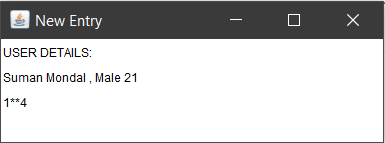
\includegraphics[width=100mm,scale=0.5]{awt/Q10.2.PNG}

\chapter{Socket Programming}
\section{TCP Socket Program}
\subproblem{socket/Q01ServerSide}{socket/Q01Server}{Server Side}
\subproblem{socket/Q01ClientSide}{socket/Q01Client}{Client Side}

\section{TCP Socket Program for Multiple Client using Threads}
\subproblem{socket/Q02ServerSide}{socket/Q02Server}{Server Side}
\subproblem{socket/Q02ClientSide}{socket/Q02Client}{Client Side}

\section{UDP Socket Program}
\subproblem{socket/Q03ServerSide}{socket/Q03Server}{Server Side}
\subproblem{socket/Q03ClientSide}{socket/Q03Client}{Client Side}

\chapter{Swing}
\problem{swing/Q01}{swing/Q01}{JPasswordField}
\problem{swing/Q02}{swing/Q02}{JTable}
\problem{swing/Q03}{swing/Q03}{JPasswordField}

\end{document}
